%% Neural pre-decoding for the surface code on four FPGA nodes
%% Author: Nasir Ali, C-DAC Noida

\documentclass[pdflatex,sn-mathphys-num]{sn-jnl}
\pdfgentounicode=1
\input{glyphtounicode}
\usepackage[T1]{fontenc}
\usepackage{lmodern}
\usepackage{graphicx}
\usepackage{multirow}
\usepackage{amsmath,amssymb,amsfonts}
\usepackage{amsthm}
\usepackage[title]{appendix}
\usepackage{xcolor}
\usepackage{textcomp}
\usepackage{manyfoot}
\usepackage{booktabs}
\usepackage[utf8]{inputenc}
\usepackage{array}
\usepackage{url}
\usepackage{etoolbox}
\AtBeginEnvironment{table}{\small}

\newcommand{\PENDING}[1]{\textcolor{red}{[PENDING: #1]}}
% generated by scripts/make_numbers.py
\newcommand{\NumCheckCount}{8}
\newcommand{\NumCheckInstances}{16}
\newcommand{\NumCheckTotal}{8}
\newcommand{\NumComputeMsAcc}{15.48}
\newcommand{\NumComputeMsFast}{3.14}
\newcommand{\NumCpuAccurateBest}{318}
\newcommand{\NumCpuAccurateBestBatch}{16}
\newcommand{\NumCpuAccurateBestThreads}{256}
\newcommand{\NumCpuAccurateOne}{114}
\newcommand{\NumCpuAccurateOneMs}{8.77}
\newcommand{\NumCpuAccurateOneThreads}{128}
\newcommand{\NumCpuFastBest}{2{,}038}
\newcommand{\NumCpuFastBestBatch}{16}
\newcommand{\NumCpuFastBestThreads}{64}
\newcommand{\NumCpuFastOne}{257}
\newcommand{\NumCpuFastOneMs}{3.89}
\newcommand{\NumCpuFastOneThreads}{32}
\newcommand{\NumCpuReps}{2}
\newcommand{\NumCpuThreadList}{32, 64, 128 and 256}
\newcommand{\NumCpuThreads}{256}
\newcommand{\NumCpuVarMaxAccurate}{108}
\newcommand{\NumCpuVarMaxFast}{95}
\newcommand{\NumCpuVarMedAccurate}{4}
\newcommand{\NumCpuVarMedFast}{12}
\newcommand{\NumCyclesAcc}{4{,}613{,}082}
\newcommand{\NumCyclesFast}{935{,}416}
\newcommand{\NumDevicePeakTmac}{5.4}
\newcommand{\NumFourAcc}{509}
\newcommand{\NumFourFast}{2{,}490}
\newcommand{\NumHlsFmax}{370}
\newcommand{\NumHostCardsAcc}{2.5}
\newcommand{\NumHostCardsFast}{3.3}
\newcommand{\NumHostCpu}{AMD EPYC 7742}
\newcommand{\NumHostMemGiB}{504}
\newcommand{\NumHostSockets}{2}
\newcommand{\NumHostThreads}{256}
\newcommand{\NumIntAccAfter}{1{,}922}
\newcommand{\NumIntAccExpected}{1{,}660}
\newcommand{\NumKernelMhz}{298}
\newcommand{\NumLatAcc}{16.56}
\newcommand{\NumLatFast}{3.77}
\newcommand{\NumLatOverheadAcc}{1.08}
\newcommand{\NumLatOverheadFast}{0.63}
\newcommand{\NumMacPerCycleAcc}{856}
\newcommand{\NumMacPerCycleFast}{711}
\newcommand{\NumMacsAcc}{3{,}948{,}272{,}640}
\newcommand{\NumMacsFast}{665{,}127{,}936}
\newcommand{\NumModelAcc}{65}
\newcommand{\NumModelEffAcc}{99}
\newcommand{\NumModelEffFast}{98}
\newcommand{\NumModelFast}{319}
\newcommand{\NumNvidiaCommit}{33acb15}
\newcommand{\NumOneAcc}{127}
\newcommand{\NumOneFast}{623}
\newcommand{\NumPerInstAcc}{64}
\newcommand{\NumPerInstFast}{311}
\newcommand{\NumPymatchingVersion}{2.4.0}
\newcommand{\NumRatioAccFpThirteenHigh}{1.72}
\newcommand{\NumRatioAccFpThirteenLow}{1.27}
\newcommand{\NumRatioAccIntThirteenHigh}{1.48}
\newcommand{\NumRatioFastFpNineHigh}{1.18}
\newcommand{\NumRatioFastFpNineLow}{1.05}
\newcommand{\NumRatioFastFpThirteenLow}{0.89}
\newcommand{\NumRatioFastIntNineHigh}{1.17}
\newcommand{\NumRatioFastIntNineLow}{1.00}
\newcommand{\NumRatioXAccFpThirteenHigh}{1.72}
\newcommand{\NumRatioXAccFpThirteenLow}{1.29}
\newcommand{\NumRatioXAccIntThirteenHigh}{1.51}
\newcommand{\NumRatioXFastFpNineHigh}{1.17}
\newcommand{\NumRatioXFastFpNineLow}{1.08}
\newcommand{\NumRatioXFastFpThirteenLow}{0.90}
\newcommand{\NumRatioXFastIntNineHigh}{1.14}
\newcommand{\NumRatioXFastIntNineLow}{0.80}
\newcommand{\NumRealTimeTmacAcc}{304}
\newcommand{\NumRealTimeTmacFast}{74}
\newcommand{\NumRealTimeWpsAcc}{76{,}923}
\newcommand{\NumRealTimeWpsFast}{111{,}111}
\newcommand{\NumScaleAcc}{1.00}
\newcommand{\NumScaleFast}{1.00}
\newcommand{\NumShotsAccFpThirteenHigh}{262{,}144}
\newcommand{\NumShotsAccFpThirteenLow}{524{,}288}
\newcommand{\NumShotsAccIntThirteenHigh}{65{,}536}
\newcommand{\NumShotsFastFpNineHigh}{1{,}048{,}576}
\newcommand{\NumShotsFastFpNineLow}{1{,}048{,}576}
\newcommand{\NumShotsFastFpThirteenLow}{1{,}048{,}576}
\newcommand{\NumShotsFastIntNineHigh}{65{,}536}
\newcommand{\NumShotsFastIntNineLow}{65{,}536}
\newcommand{\NumSpeedAcc}{1.6}
\newcommand{\NumSpeedFast}{1.2}
\newcommand{\NumStimVersion}{1.16.0}
\newcommand{\NumTempMax}{83}
\newcommand{\NumTmacAcc}{2.01}
\newcommand{\NumTmacFast}{1.66}
\newcommand{\NumTorchVersion}{2.14.1}
\newcommand{\NumUtilBram}{269}
\newcommand{\NumUtilDsp}{1{,}296}
\newcommand{\NumUtilLut}{38{,}496}
\newcommand{\NumUtilReg}{50{,}553}
\newcommand{\NumUtilUram}{114}
\newcommand{\NumWns}{-0.013}
\newcommand{\NumXrtVersion}{2.16.204}


\raggedbottom

\begin{document}

\title[Neural Pre-Decoding on Four FPGA Nodes]{Neural Pre-Decoding for the Surface Code on Four FPGA Nodes:
Integer Inference of Convolutional Pre-Decoders on Alveo U55C Accelerators}

\author*[1]{\fnm{Nasir} \sur{Ali}}\email{nasirali2607@gmail.com}

\affil*[1]{\orgdiv{Embedded Systems Division},
           \orgname{Centre for Development of Advanced Computing},
           \orgaddress{\city{Noida}, \postcode{201307}, \country{India}}}

\abstract{Neural pre-decoders remove local errors from the syndrome of a quantum error correcting code before a global decoder
such as matching processes the remainder. We implement the two surface code pre-decoders that
NVIDIA released with pretrained weights, four and six layer three dimensional convolutional networks, as integer
networks on four AMD Alveo U55C FPGA cards, each card an independent node with two instances of one HLS kernel that
runs both networks. The kernel uses 8 bit products, 32 bit accumulation and a table based GELU, keeps all activations
on chip, and is bit exact with an integer model of the networks on every instance of every card. Measured with
NVIDIA's evaluation code, the six layer network lowers the logical error rate of matching by a factor of
\NumRatioAccFpThirteenHigh{} at physical error rate 0.006 and distance 13, as published, and the integer model by
\NumRatioAccIntThirteenHigh{}, while the four layer network gives little or no gain at
0.003. Four cards process \NumFourFast{} windows per second of the four layer network at distance 9 and
\NumFourAcc{} of the six layer network at distance 13, with linear scaling and within two percent of the kernel schedule,
but only \NumSpeedFast{} and \NumSpeedAcc{} times the same networks in PyTorch on
a 256 thread host CPU. A single window takes \NumLatFast{} and \NumLatAcc{} milliseconds, no faster than on the CPU. The arithmetic per window shows
that real time pre-decoding at microsecond syndrome cycles requires networks designed for hardware, while the cards
offload batch evaluation from the host.
}

\keywords{FPGA, Quantum error correction, Surface code, Neural decoder, Pre-decoder, Integer quantization,
High-level synthesis, Multi-FPGA, Alveo U55C}

\maketitle

\section{Introduction}\label{sec:intro}

A fault tolerant quantum computer protects its logical qubits with an error correcting code and must decode the
syndrome of that code while the computation runs \cite{dennis2002topological,fowler2012surface}. The rotated surface
code \cite{kitaev2003anyons,fowler2012surface} is the leading candidate for superconducting hardware, where logical memories below threshold have now been
demonstrated \cite{google2023scaling,google2025below}. Its standard decoder, minimum weight perfect matching, is
implemented efficiently on CPUs by PyMatching and the Sparse Blossom algorithm \cite{higgott2022pymatching,
higgott2025sparse}, and union find decoders trade some accuracy for a simpler and faster procedure
\cite{delfosse2021unionfind}. Because a superconducting device produces a new round of syndrome data about every
microsecond, a decoder that falls behind accumulates a backlog that eventually stalls the computation, and dedicated
hardware such as FPGAs has been used to keep up \cite{das2022lilliput,liyanage2023fpga,liyanage2024distributed,
barber2025decoder}. Where syndrome cycles last milliseconds, as in trapped ion architectures, a single CPU can decode
all logical qubits of a large application in real time \cite{ye2026megaquop}; the case for accelerators therefore
rests on the microsecond budget of fast platforms.

Neural networks offer a second route. They have been trained as complete decoders \cite{torlai2017neural,
chamberland2018deep,gicev2023scalable,bausch2024alphaqubit} and, more recently, as \emph{pre-decoders}: a local
network removes the short error chains that dominate the syndrome and leaves a sparser residual syndrome to a global
decoder. Chamberland et al.\ released a family of such pre-decoders, the NVIDIA Ising pre-decoders, as fully
convolutional three dimensional networks over space and time, together with their training code and pretrained
weights \cite{chamberland2026predecoder,nvidia_ising_code,nvidia_fast_card,nvidia_accurate_card}. On GPUs the
pre-decoder both lowers the logical error rate of uncorrelated matching and shortens the time PyMatching needs for the
residual syndrome \cite{chamberland2026predecoder}. A convolutional network of fixed size, applied to a fixed window of
syndrome data, is also a natural workload for an FPGA: its arithmetic is regular, its weights fit on chip, and
integer arithmetic suffices for inference \cite{jacob2018quantization,zhang2015optimizing,umuroglu2017finn,
duarte2018hls4ml}. Overwater et al.\ analysed the hardware cost of neural decoders for this reason
\cite{overwater2022neural}.

This paper places the two published surface code pre-decoders on four AMD Alveo U55C cards. Following our earlier
multi FPGA work, each card is an independent compute node driven by its own host process \cite{ali2026multifpga}; a
batch of syndrome windows is spread over the nodes, which is the shot parallel mode of a decoder serving many
independent windows. The contributions are:

\begin{itemize}
\item An integer model of both networks (8 bit weights and activations, 32 bit accumulation, integer requantization
and a 256 entry GELU table) that keeps NVIDIA's evaluation pipeline unchanged, so that the floating point networks,
the integer model and the FPGA output are judged by the same logical error rate code.
\item One HLS kernel that runs the four layer Fast network and the six layer Accurate network from the same bitstream,
with all activations and partial sums on chip, and that is bit exact with the integer model in C simulation and on
every instance of every card.
\item Measurements on four cards: throughput on one, two and four nodes and latency per window, against the same
networks in PyTorch on a 256 thread host CPU, and logical error rates of the floating point and integer networks
against PyMatching alone.
\item A reproduction of NVIDIA's published accuracy for both networks with their own evaluation code, which shows when a
pre-decoder pays off: the small Fast network gives little or no gain at a physical error rate of $p=0.003$, and the
gains reported for the family come from the larger network and from higher noise.
\end{itemize}

Section~\ref{sec:related} reviews decoders on FPGAs and neural decoders, Section~\ref{sec:background} the
pre-decoder and its evaluation, Section~\ref{sec:quant} the integer model, Section~\ref{sec:arch} the kernel and the
node runtime, Section~\ref{sec:setup} the experimental setup, Section~\ref{sec:results} the results and
Section~\ref{sec:discussion} their limits.

\section{Related work}\label{sec:related}

\textbf{Decoders on FPGAs.} LILLIPUT maps small surface codes to lookup tables in FPGA memory \cite{das2022lilliput}.
Liyanage et al.\ implemented a union find decoder for surface codes on an FPGA and later proposed a
distributed union find decoder \cite{liyanage2023fpga,liyanage2024distributed}. Barber et al.\ demonstrated a real time, resource efficient decoder in
FPGA and ASIC form \cite{barber2025decoder}. These designs implement a complete decoder in custom logic; the present
work instead accelerates a learned stage in front of an unchanged software decoder.

\textbf{Neural decoders.} Torlai and Melko trained a restricted Boltzmann machine as a decoder for topological codes
\cite{torlai2017neural}. Chamberland and Ronagh studied deep neural decoders for fault tolerance experiments and noted
the latency constraints of real time use \cite{chamberland2018deep}. Gicev et al.\ proposed a convolutional decoder
that scales to large distances \cite{gicev2023scalable}, and AlphaQubit learned a high accuracy decoder from
experimental data \cite{bausch2024alphaqubit}. Overwater et al.\ explored the trade off between hardware cost and
performance of neural network decoders for the surface code \cite{overwater2022neural}.

\textbf{Pre-decoders.} The NVIDIA Ising pre-decoders \cite{chamberland2026predecoder} are fully convolutional
networks over a space and time window of the syndrome. They predict local data qubit corrections and syndrome flips;
after the corrections are applied, PyMatching decodes the residual syndrome. Five surface code models of growing size
are described; two are released with weights, the four layer model 1 (``Fast'', receptive field 9) and the six layer
model 4 (``Accurate'', receptive field 13) \cite{nvidia_fast_card,nvidia_accurate_card}. Their reference
implementation targets GPUs and TensorRT, including reduced precision inference.

\textbf{Neural networks on FPGAs.} Weight stationary convolution engines with on chip buffers are the classic FPGA
design for convolutional networks \cite{zhang2015optimizing}; FINN and hls4ml generate quantized network accelerators
from high level descriptions \cite{umuroglu2017finn,duarte2018hls4ml}, and integer only inference with per channel
scales and requantization multipliers is the standard quantization scheme \cite{jacob2018quantization}. Our kernel
follows these principles in hand written HLS \cite{cong2011hls,amd_ug1399} so that its arithmetic matches an integer
model that can be checked against NVIDIA's evaluation.

\textbf{Multiple FPGAs as nodes.} In our earlier work a quantum circuit statevector was distributed over four Alveo
U55C cards, each card a node with its own host process and memory \cite{ali2026multifpga}. The same view applies
here, without data exchange between cards because the windows are independent.

\section{The Ising pre-decoders and their evaluation}\label{sec:background}

\textbf{Input window.} The pre-decoder sees a window of $T$ syndrome rounds of a rotated surface code of distance $d$
as a tensor of shape $(4, T, d, d)$ \cite{chamberland2026predecoder}. Two channels carry the syndrome bits of the X
and Z stabilizers, placed on the $d\times d$ grid of data qubits, and two channels carry fixed masks that mark which
grid positions hold a stabilizer of each type. The syndrome channels take the values 0 and 1 and the mask channels
the values 0, $\tfrac12$ and 1.

\textbf{Network.} Both released surface code networks are stacks of three dimensional convolutions with $3\times
3\times 3$ kernels, zero padding that keeps the window size, and the tanh approximation of GELU
\cite{hendrycks2016gelu} between layers, without normalization layers. The Fast network (model 1) has four layers,
$4\to128\to128\to128\to4$ channels and 912{,}772 parameters; the Accurate network (model 4) has six layers,
$4\to128\to128\to128\to128\to128\to4$ channels and about 1.8 million parameters \cite{nvidia_fast_card,
nvidia_accurate_card}. Their receptive fields are 9 and 13 sites, and they were trained on windows with $d=T=9$ and
$d=T=13$. Because the networks are fully convolutional, the same weights apply to any larger window.

\textbf{Output and use.} The four output channels are logits of a correction on each data qubit (two channels) and
of a flip of each syndrome bit (two channels). A logit at or above a threshold (zero in the released configuration)
selects the correction. The corrections are applied to the syndrome, and PyMatching decodes the residual syndrome
with the detector error model of the circuit; the logical outcome combines the pre-decoder corrections and the
matching \cite{chamberland2026predecoder,higgott2025sparse}.

\textbf{Evaluation.} NVIDIA's evaluation samples memory experiments with Stim \cite{gidney2021stim} under a circuit
level noise model with 25 parameters (state preparation, measurement, idling during CNOT layers and during
preparation and reset, and the fifteen two qubit Pauli errors of a CNOT), which their public configuration sets for a
physical error rate $p=0.003$ \cite{nvidia_ising_code}. For each shot it reports whether PyMatching alone and the
pre-decoder followed by PyMatching recover the logical observable. We use this code without modification for every
logical error rate in this paper, and add only the scaling of the 25 parameters to other values of $p$ with the
relations given in the public configuration (preparation and measurement $2p/3$, idling during CNOT layers $p/3$ per
Pauli, idling during preparation and reset $2p/3-4p^2/9$ per Pauli, and $p/15$ per two qubit Pauli). We report the
ratio of the number of logical errors of PyMatching alone to that of the pre-decoder followed by PyMatching on the
same shots; a ratio above one is an improvement.

\section{Integer model}\label{sec:quant}

The FPGA kernel computes an integer model of the network, defined in software first so that it can be judged by
NVIDIA's evaluation and so that the kernel can be checked against it bit for bit.

\textbf{Inputs.} Multiplying the input tensor by two maps every entry to $\{0,1,2\}$, so the input is exact in
integers with scale $\tfrac12$; a site of the window needs two bits per channel, eight bits for its four channels.

\textbf{Weights.} The weights of each output channel are scaled to integers in $[-127,127]$ with a per channel scale, the
largest absolute weight of the channel divided by 127
\cite{jacob2018quantization}, and the biases are rounded to 32 bit integers at the scale of the accumulator, so that a
layer computes $a_o = b_o + \sum_{i,\tau} w_{o i \tau}\, x_{i}(\text{site}+\tau)$ exactly in a 32 bit accumulator over
the 27 kernel offsets $\tau$ and the input channels $i$.

\textbf{Requantization and activation.} For a hidden layer, the accumulator is mapped to an 8 bit index
\begin{equation}
q_o = \operatorname{clamp}\bigl(\lfloor (a_o M_o + 2^{23}) / 2^{24} \rfloor,\, -128,\, 127\bigr),
\end{equation}
with a per channel integer multiplier $M_o$, and the activation of the next layer is $g[q_o]$, a 256 entry table of
signed 8 bit values that holds the GELU of the dequantized index at the scale of the next layer. The multipliers and
the table scales come from calibration: the 99.99th percentile of the absolute values of each layer's floating point pre-activations on
syndrome windows of NVIDIA's inference pipeline sets the range of the index, and the same percentile of the
activations sets the scale of the table output.

\textbf{Decision.} The last layer needs no requantization: a logit is at or above the threshold exactly when the
accumulator is at or above the threshold divided by the accumulator scale, rounded up, so the kernel compares the
32 bit accumulator with an integer threshold per output channel and emits one bit.

\textbf{Reference implementations.} The integer model has a direct implementation in NumPy and a fast one that
evaluates the convolutions in double precision, which represents every 32 bit accumulator exactly; the two agree bit
for bit. The fast path supplies the network inside NVIDIA's evaluation module, in place of the floating point network,
to obtain the logical error rate of the integer model.

\section{Kernel and node runtime}\label{sec:arch}

\subsection{Convolution engine}

The kernel is written in C++ for Vitis HLS \cite{amd_ug1399} and processes one window at a time through all layers
of the network on a single convolution engine (Fig.~\ref{fig:kernel}). It stores the activations of a window on chip
in two buffers that alternate between layers, each holding 128 channels of 8 bit values for up to
$13\times13\times13$ sites, so that no intermediate result leaves the FPGA. The engine is weight stationary
\cite{zhang2015optimizing}: for a block of 64 output channels it keeps the 32 bit partial sums of every site on chip;
for each of the 27 kernel offsets and each block of 16 input channels it loads a $64\times16$ block of 8 bit weights
into registers and streams all sites of the window through the engine, one site per clock cycle. At each site the
engine reads the 16 input activations of the neighbour at the kernel offset (zero outside the window, which realizes
the zero padding of the network) and adds 1024 products to the 64 partial sums. After the last offset and input
block, an epilogue pipeline adds the biases and either requantizes and maps the 64 results through the GELU table
(hidden layers) or compares them with the thresholds and writes one bit per output channel (last layer). The weights
of all layers stay in UltraRAM for the lifetime of the kernel and are loaded from HBM once per launch.

\begin{figure}[t]
\centering
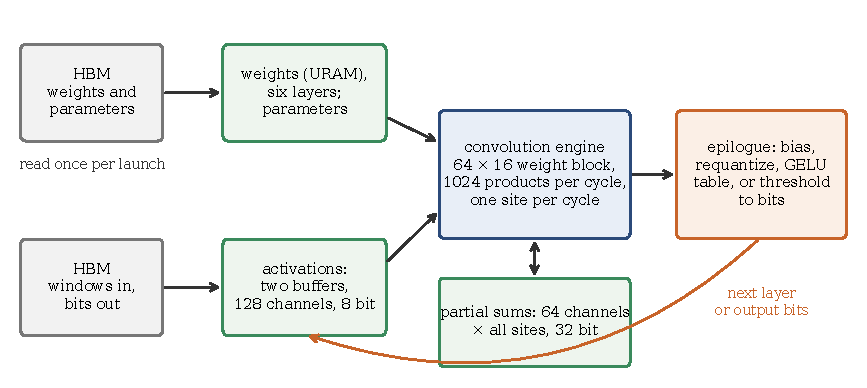
\includegraphics[width=\textwidth]{figures/fig_kernel.pdf}
\caption{Kernel of one instance. Weights and parameters are read from HBM into on chip memories once per launch. For
each window, the convolution engine runs the layers one after the other; activations alternate between two on chip
buffers, and the partial sums of 64 output channels stay on chip for all sites. Each card holds two instances, in SLR1
and SLR2.}\label{fig:kernel}
\end{figure}

\subsection{Epilogue parameters}

A first version read the bias, multiplier and table entry of each of the 64 output channels per cycle from one
parameter memory, at addresses that depend on the layer. HLS partitioned that memory into 144 banks and had not finished
scheduling the epilogue when it was stopped after 7{,}000 seconds. The final kernel copies each layer's biases, multipliers and thresholds
into registers and its activation table into 64 small per channel memories before the sites stream through, so the
epilogue reads every parameter at a fixed lane. With this change C synthesis finishes in about two minutes, every
loop of the engine and epilogue reaches an initiation interval of one, and the estimated maximum clock frequency is
\NumHlsFmax{}~MHz against the 300~MHz target.

\subsection{One bitstream for both networks}

Both networks have 128 hidden channels and differ only in the number of layers, so the layer count is a launch
argument (four or six) and the on chip weight and parameter memories are sized for six layers. The host derives the
layer count from the size of the parameter file; the kernel reads only the weights and parameters of the layers the
host supplies. One bitstream therefore runs the Fast network and the Accurate network.

\subsection{Throughput model}

The work per window is fixed by the network and the window size: $\NumMacsFast$ multiply accumulate operations for the
Fast network at $d=T=9$ and $\NumMacsAcc$ for the Accurate network at $d=T=13$. From the loop structure and the
pipeline depths reported by HLS, a window takes $\NumCyclesFast$ cycles (Fast, $d=9$) or $\NumCyclesAcc$ cycles
(Accurate, $d=13$) on one instance, that is $\NumMacPerCycleFast$ and $\NumMacPerCycleAcc$ useful operations per cycle
out of the 1024 the engine can perform. The difference to the peak comes from the first layer, which has four input
channels on an engine built for 16, the last layer, which has four output channels on an engine built for 64, and the
pipeline fill at each kernel offset. At 300~MHz the model predicts $\NumModelFast$ windows per second per instance for
the Fast network at $d=9$ and $\NumModelAcc$ for the Accurate network at $d=13$.

\subsection{Cards as nodes}

Each card carries two kernel instances, placed in SLR1 and SLR2 because SLR0 also holds the platform's HBM and DMA
logic; each instance has its own two HBM pseudo channels, one for weights and parameters and one for windows and
output bits. As in our multi FPGA statevector work \cite{ali2026multifpga}, every card is a node driven by its own host
process through XRT \cite{amd_xrt}. A process loads the bitstream, copies the weights and parameters to both
instances once, and then keeps two launches per instance in flight so that the transfer of one batch of windows
overlaps the computation of the previous one. For multi card runs all processes finish their setup, wait at a common
start barrier, and report the wall clock interval of their timed loop; the aggregate throughput is the total number of
windows divided by the interval from the first start to the last end. The windows of a batch are independent, so the
nodes exchange no data.

\section{Experimental setup}\label{sec:setup}

\textbf{Hardware.} The host has two \NumHostCpu{} processors with \NumHostThreads{} hardware threads in total and
\NumHostMemGiB{}~GiB of memory, and four AMD Alveo U55C cards \cite{amd_ds978} on PCIe, each with 16~GiB of HBM2 and the
shell \texttt{xilinx\_u55c\_gen3x16\_xdma\_base\_3}, driven by XRT \NumXrtVersion{} \cite{amd_xrt}. The kernel was
synthesized with Vitis HLS 2023.2 and linked with Vitis 2023.2 at a 300~MHz kernel clock target, with the two instances
constrained to SLR1 and SLR2.

\textbf{Networks and evaluation.} The pretrained Fast (checkpoint v1.0.77) and Accurate (v1.0.86) networks were
downloaded from NVIDIA's model pages and checked against their published SHA256 hashes \cite{nvidia_fast_card,
nvidia_accurate_card}. Logical error rates were computed with NVIDIA's evaluation code at commit \NumNvidiaCommit{}
\cite{nvidia_ising_code}, run on the host CPU with PyTorch \NumTorchVersion{}, Stim \NumStimVersion{}
\cite{gidney2021stim} and PyMatching \NumPymatchingVersion{} \cite{higgott2025sparse}, for memory experiments in both
the X and the Z basis with $T=d$ rounds. The integer model was calibrated on 2{,}048 windows (Fast) or 1{,}024 windows
(Accurate), half from each basis, drawn from the same pipeline at the same noise level, separate from the
evaluation shots.

\textbf{Card measurements.} Each card measurement starts with a bit exact check: a batch of windows from the
inference pipeline (eight test windows, after a calibration of the integer model on 256 other windows) runs on both
instances of every card, and the output bits are compared with the integer model.
Throughput is then measured on one, two and four cards with batches of 64 windows per launch, two launches in flight
per instance, and about 20 seconds per point, three repetitions per point; we report the median. Latency is the time
of one launch of a single window with one launch in flight, averaged over 200 launches; it includes the host to card
transfer of the window and the transfer of the result back. The card temperatures are read before and after every
point. A logical error rate evaluation ran on the host CPU during the card measurements; the host
processes of the cards only start launches and copy data, and the throughput agrees with the cycle model of the
kernel (Section~\ref{sec:hw}).

\textbf{CPU baseline.} The same floating point networks run in PyTorch \NumTorchVersion{} on the host, in inference
mode, with the cards idle and no other job running, with \NumCpuThreadList{} threads and batch sizes from 1 to 256,
each point for 10 seconds and repeated \NumCpuReps{} times. We report the best throughput over threads, batch sizes
and repetitions, and the best throughput at batch size one; on this two socket host fewer threads are often faster
than all of them. Reduced precision (bfloat16) was much slower than single precision on this processor and is not
used.

\section{Results}\label{sec:results}

\subsection{Logical error rates}

Table~\ref{tab:ler} lists the logical errors of PyMatching alone and of the pre-decoder followed by PyMatching on the
same shots, for both networks, both noise levels and both arithmetics, together with the improvement factors NVIDIA
published for the X basis \cite{chamberland2026predecoder}; Fig.~\ref{fig:ler} compares the X basis factors.

\begin{table}[t]
\caption{Logical errors over both bases (X and Z, each with the stated number of shots) of PyMatching alone and of
the pre-decoder followed by PyMatching on the same shots, with $T=d$ rounds. Ratio, X: improvement factor in the X
basis (PyMatching errors divided by errors with the pre-decoder); NVIDIA, X: the published factor for the same
network, $p$ and $d$ (Tables 4 and 5 of \cite{chamberland2026predecoder}).}\label{tab:ler}
\centering
% generated by scripts/make_numbers.py
\begin{tabular}{@{}llrrrrrrr@{}}
\toprule
Network & Arithmetic & $d$ & $p$ & Shots per basis & PyMatching & With pre-decoder & Ratio, X & NVIDIA, X \\
\midrule
Fast & FP32 & 9 & 0.003 & 1{,}048{,}576 & 2{,}605 & 2{,}479 & 1.08 & 1.10 \\
Fast & INT8 & 9 & 0.003 & 65{,}536 & 154 & 154 & 0.80 & 1.10 \\
Fast & FP32 & 13 & 0.003 & 1{,}048{,}576 & 519 & 586 & 0.90 & 0.91 \\
Fast & FP32 & 9 & 0.006 & 1{,}048{,}576 & 61{,}392 & 51{,}883 & 1.17 & 1.24 \\
Fast & INT8 & 9 & 0.006 & 65{,}536 & 3{,}887 & 3{,}317 & 1.14 & 1.24 \\
Accurate & FP32 & 13 & 0.003 & 524{,}288 & 223 & 176 & 1.29 & 1.32 \\
Accurate & FP32 & 13 & 0.006 & 262{,}144 & 11{,}577 & 6{,}747 & 1.72 & 1.76 \\
Accurate & INT8 & 13 & 0.006 & 65{,}536 & 2{,}849 & 1{,}922 & 1.51 & 1.76 \\
\botrule
\end{tabular}

\end{table}

\begin{figure}[t]
\centering
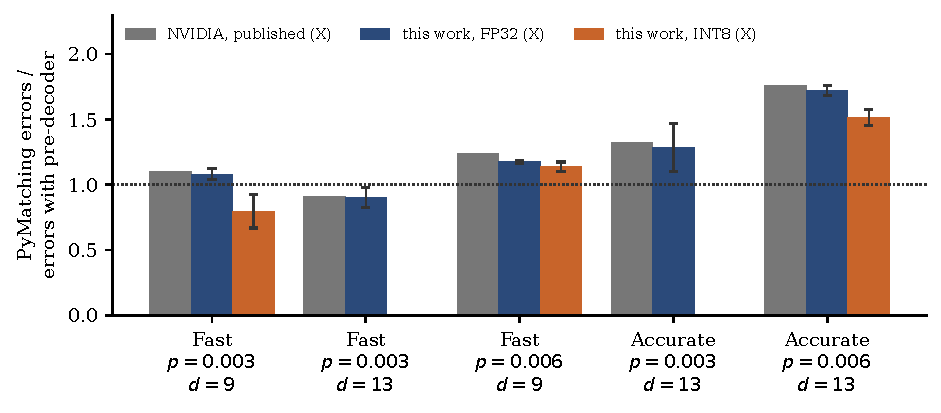
\includegraphics[width=\textwidth]{figures/fig_ler.pdf}
\caption{Improvement factor of the pre-decoder over PyMatching alone in the X basis: NVIDIA's published values and
the values measured here with NVIDIA's evaluation code, for the floating point (FP32) and the integer (INT8)
networks. Error bars: one standard deviation from the counts of logical errors. Values below the dotted line mean
that the pre-decoder increases the logical error rate.}\label{fig:ler}
\end{figure}

\textbf{Agreement with the published values.} With NVIDIA's own evaluation code our measurements follow the published
factors in the X basis. The Fast network at $p=0.003$ gives \NumRatioXFastFpNineLow{} at $d=9$ and
\NumRatioXFastFpThirteenLow{} at $d=13$ (\NumShotsFastFpThirteenLow{} shots per basis each), against 1.10 and 0.91
published, and at $p=0.006$, $d=9$ \NumRatioXFastFpNineHigh{} (\NumShotsFastFpNineHigh{} shots per basis), against
1.24. The Accurate network at $d=13$ gives \NumRatioXAccFpThirteenLow{} at $p=0.003$ (\NumShotsAccFpThirteenLow{} shots
per basis) and \NumRatioXAccFpThirteenHigh{} at $p=0.006$ (\NumShotsAccFpThirteenHigh{} shots per basis), against 1.32
and 1.76. Every factor we measure is within 0.07 of the published one and slightly below it.

\textbf{When the pre-decoder pays off.} The small Fast network gives at best a modest gain: at $p=0.003$ it lowers the
logical error rate by a factor of only \NumRatioFastFpNineLow{} over both bases at $d=9$ and raises it at $d=13$
(\NumRatioFastFpThirteenLow{}), in agreement with the factor below one that NVIDIA reports for this network at this
noise level. The Accurate network, with two more layers and a receptive field
of 13, lowers the logical error rate by a factor of \NumRatioAccFpThirteenHigh{} over both bases at $p=0.006$ and by
\NumRatioAccFpThirteenLow{} at $p=0.003$, both at $d=13$. The gains quoted for the network family therefore depend on
the network size and the noise level, and a hardware implementation should target the larger network.

\textbf{Integer arithmetic.} The integer model of the Fast network gives a factor of \NumRatioFastIntNineHigh{} over
both bases at $p=0.006$, $d=9$ (\NumShotsFastIntNineHigh{} shots per basis), against \NumRatioFastFpNineHigh{} in
floating point, and the integer Accurate network gives \NumRatioAccIntThirteenHigh{} at $p=0.006$, $d=13$
(\NumShotsAccIntThirteenHigh{} shots per basis), against \NumRatioAccFpThirteenHigh{}. The integer model thus keeps
the gain of the four layer network but loses about a third of the gain of the six layer network, plausibly because the rounding of
the activations accumulates over five hidden layers; with \NumIntAccAfter{} errors against \NumIntAccExpected{}
expected on the same shots from the floating point factor, the loss is well outside the counting uncertainty. At $p=0.003$, $d=9$ the integer Fast network gives
\NumRatioFastIntNineLow{} over both bases, with too few errors (\NumShotsFastIntNineLow{} shots per basis) to
distinguish it from the floating point network. Since the kernel output is bit exact with the integer model
(Section~\ref{sec:hw}), these are the logical error rates the cards deliver.

\subsection{Hardware}\label{sec:hw}

\textbf{Implementation.} After routing and post route physical optimization, the two instance design misses the
300~MHz target by a worst negative slack of \NumWns{}~ns, and Vitis lowers the kernel clock to \NumKernelMhz{}~MHz. Table~\ref{tab:resources} lists the routed resources of one
instance. The routed design uses more DSP blocks and BRAM and fewer URAM blocks than the HLS estimate, because the
implementation maps part of the products to DSP blocks and part of the on chip memories to BRAM; DSP blocks are the
largest share, at less than half of one SLR.

\begin{table}[t]
\caption{Routed resources of one kernel instance (the second instance is within 2\% of these values), as reported
by Vivado after implementation, and their share of one SLR of the U55C.}\label{tab:resources}
\centering
% generated by scripts/make_numbers.py
\begin{tabular}{@{}lrr@{}}
\toprule
Resource & One instance & Percent of one SLR \\
\midrule
LUT & 38{,}496 & 8.9 \\
Flip flops & 50{,}553 & 5.8 \\
DSP blocks & 1{,}296 & 43.1 \\
BRAM (36 kbit) & 269 & 40.0 \\
URAM & 114 & 35.6 \\
\botrule
\end{tabular}

\end{table}

\textbf{Bit exactness.} All \NumCheckCount{} checks (two networks on four cards) passed: the output bits of all \NumCheckInstances{} instance runs equal those of the integer model for every site
and output channel of the test windows. Since the kernel computes the integer model exactly for any calibration, the logical error rates of the integer
model in Table~\ref{tab:ler} are those of the cards.

\textbf{Throughput.} Table~\ref{tab:throughput} and Fig.~\ref{fig:throughput} give the measured throughput. One card
processes \NumOneFast{} windows per second of the Fast network at $d=9$ and \NumOneAcc{} of the Accurate network at
$d=13$, and four cards \NumFourFast{} and \NumFourAcc{}: the scaling from one to four cards is \NumScaleFast{} and
\NumScaleAcc{}, as expected for nodes that exchange no data, and the three repetitions of each point agree to within
one window per second. One instance reaches \NumModelEffFast{}\% (Fast) and \NumModelEffAcc{}\% (Accurate) of the
throughput predicted by the cycle model at \NumKernelMhz{}~MHz, so the transfers of the windows and of the output bits
are hidden behind the computation and the kernel runs at the rate its schedule allows. In products per second, four
cards perform \NumTmacFast{}$\times10^{12}$ (Fast) and \NumTmacAcc{}$\times10^{12}$ (Accurate) useful 8 bit
multiply accumulate operations per second. During the measurements the card temperatures stayed at or below
\NumTempMax{}~$^\circ$C.

\begin{table}[t]
\caption{Throughput in windows per second on one, two and four cards (two instances per card), median and range of
three repetitions of about 20 seconds each. Scaling: throughput divided by the number of cards times the throughput of
one card.}\label{tab:throughput}
\centering
% generated by scripts/make_numbers.py
\begin{tabular}{@{}lrrrrr@{}}
\toprule
Network & Cards & Windows/s (median) & Range & Per card & Scaling \\
\midrule
Fast, $d=9$ & 1 & 623 & 622 to 623 & 623 & 1.00 \\
Fast, $d=9$ & 2 & 1{,}245 & 1{,}245 to 1{,}245 & 622 & 1.00 \\
Fast, $d=9$ & 4 & 2{,}490 & 2{,}490 to 2{,}490 & 622 & 1.00 \\
\midrule
Accurate, $d=13$ & 1 & 127 & 127 to 127 & 127 & 1.00 \\
Accurate, $d=13$ & 2 & 255 & 255 to 255 & 127 & 1.00 \\
Accurate, $d=13$ & 4 & 509 & 509 to 509 & 127 & 1.00 \\
\botrule
\end{tabular}

\end{table}

\begin{figure}[t]
\centering
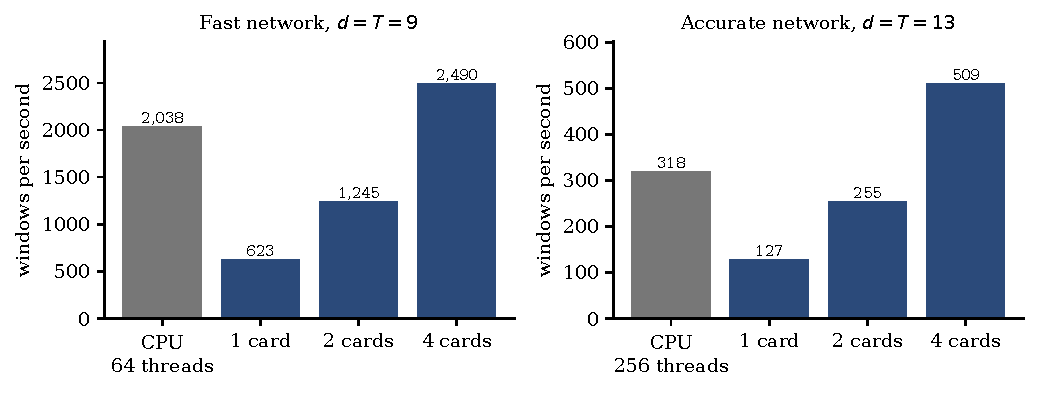
\includegraphics[width=\textwidth]{figures/fig_throughput.pdf}
\caption{Throughput of the floating point networks in PyTorch on the host CPU (best thread count and batch size) and of
the integer networks on one, two and four cards.}\label{fig:throughput}
\end{figure}

\textbf{Comparison with the host CPU.} PyTorch on the host reaches at best \NumCpuFastBest{} windows per second for
the Fast network (\NumCpuFastBestThreads{} threads, batch size \NumCpuFastBestBatch{}) and \NumCpuAccurateBest{} for
the Accurate network (\NumCpuAccurateBestThreads{} threads, batch size \NumCpuAccurateBestBatch{}); at batch size one
it reaches \NumCpuFastOne{} and \NumCpuAccurateOne{}, that is \NumCpuFastOneMs{}~ms and \NumCpuAccurateOneMs{}~ms per
window. Four cards are therefore only \NumSpeedFast{} times (Fast) and \NumSpeedAcc{} times (Accurate) faster than the
host CPU at its best setting, and one card is slower than the host. The throughput of the CPU varies between the two
repetitions of a point, by a median of \NumCpuVarMedFast{}\% (Fast) and \NumCpuVarMedAccurate{}\% (Accurate) and by up
to \NumCpuVarMaxAccurate{}\% at single points; the comparison uses the best repetition, which favours the CPU.

\textbf{Latency.} With one window per launch and one launch in flight, a window takes \NumLatFast{}~ms (Fast, $d=9$)
and \NumLatAcc{}~ms (Accurate, $d=13$) from the start of the transfer to the card until its bits are back on the host.
The computation alone takes \NumComputeMsFast{}~ms and \NumComputeMsAcc{}~ms according to the cycle model; the
remaining \NumLatOverheadFast{}~ms and \NumLatOverheadAcc{}~ms cover the transfers, the kernel launch through XRT and
the loading of the weights from HBM, which each launch repeats.

\section{Discussion}\label{sec:discussion}

\textbf{Distance to real time decoding.} A superconducting device produces a syndrome round about every microsecond
\cite{google2025below}. To keep up with one logical qubit, a pre-decoder that consumes windows of $T=d$ rounds must
finish at least one window every $d$ microseconds: \NumRealTimeWpsFast{} windows per second for the Fast network at
$d=9$ and \NumRealTimeWpsAcc{} for the Accurate network at $d=13$. Because the work per window is fixed, this asks for
\NumRealTimeTmacFast{}$\times10^{12}$ and \NumRealTimeTmacAcc{}$\times10^{12}$ multiply accumulate operations per
second. Four cards deliver \NumTmacFast{}$\times10^{12}$ and \NumTmacAcc{}$\times10^{12}$, and even if every one of the
9{,}024 DSP blocks of a U55C \cite{amd_ds978} performed two 8 bit products per cycle at 300~MHz, one card would reach
\NumDevicePeakTmac{}$\times10^{12}$. The released networks evaluated densely on full windows therefore need more than ten
times the peak arithmetic of a card of this class for real time use, independently of how well the engine is
scheduled; our kernel already reaches \NumModelEffFast{}\% and \NumModelEffAcc{}\% of the rate its schedule allows. The
measured latency of \NumLatFast{}~ms per window leads to the same conclusion. Real time pre-decoding in hardware
therefore needs networks designed for it: fewer channels, fewer layers, or sliding windows that reuse the results of
earlier rounds instead of recomputing a full window, and possibly the sparsity of the syndrome, which in our kernel
only the first layer could exploit because the hidden activations after GELU are dense. On platforms with millisecond
syndrome cycles, a CPU already decodes in real time \cite{ye2026megaquop}, and a pre-decoder is not needed for speed.

\textbf{What the cards are useful for.} The design is a throughput engine. Evaluating a pre-decoder on many shots, as
in Table~\ref{tab:ler}, and generating pre-decoded syndromes for decoder studies are batch tasks of independent windows,
which spread over the cards without communication and scale linearly with their number. For these tasks, however,
the advantage of the cards over the host is small: four cards are \NumSpeedFast{} (Fast) and \NumSpeedAcc{}
(Accurate) times faster than PyTorch on the two socket, 128 core host at its best thread count and batch size, so the
host matches \NumHostCardsFast{} cards for the Fast network and \NumHostCardsAcc{} for the Accurate network, and for a single window the CPU is as fast (Fast) or faster (Accurate). What the cards
offer is that the work leaves the host, whose cores then remain free for the matching decoder, and an integer output
known to be bit exact. The CPU baseline is the floating point network in PyTorch, the form in which the networks are
released; an optimized integer CPU implementation could close or reverse the remaining gap, and we did not measure GPUs
or the power of either platform. The per card throughput is limited by the single engine of 1{,}024 products per cycle
per instance, which uses less than half of the DSP blocks of an SLR (Table~\ref{tab:resources}); a larger engine or
two products per DSP block would raise it, but not by the factor that real time use needs.

\textbf{Accuracy of the integer model.} The integer model keeps the gain of the Fast network and about two thirds of
that of the Accurate network: the Fast network at $p=0.006$, $d=9$ gives \NumRatioFastIntNineHigh{} against \NumRatioFastFpNineHigh{}, and the Accurate
network at $p=0.006$, $d=13$ gives \NumRatioAccIntThirteenHigh{} against \NumRatioAccFpThirteenHigh{}, both over both
bases. Calibration uses windows of both bases at the noise level of the evaluation and no retraining; quantization aware
training could recover the remainder.

\textbf{Limits of this study.} The kernel holds windows up to $13\times13\times13$ sites and the two released surface
code networks; larger windows need tiling of the activation buffers. Every launch reloads the weights from HBM, which
costs little in throughput but adds to the latency of a single window; a kernel that keeps the weights resident between
launches would remove that part. Logical error rates are measured for memory experiments under NVIDIA's circuit level
noise model at two noise levels, with the number of shots given in Table~\ref{tab:ler}; the smallest counts, at
$p=0.003$, carry a relative statistical uncertainty of up to about ten percent.

\section{Conclusions}\label{sec:conclusions}

We implemented the two released NVIDIA Ising surface code pre-decoders as one integer HLS kernel on four Alveo U55C
cards, each card a node with two kernel instances. The kernel is bit exact with an integer model of the networks on
every instance of every card, and the integer model is evaluated with NVIDIA's unmodified evaluation code. With that
code we reproduce the published accuracy of both networks: the Accurate network lowers the logical error rate of
PyMatching by a factor of \NumRatioAccFpThirteenHigh{} at $p=0.006$, $d=13$, while the Fast network gives little or no
gain at $p=0.003$. Four cards process \NumFourFast{} windows per second of the Fast network at $d=9$ and \NumFourAcc{}
of the Accurate network at $d=13$, with linear scaling over the cards and \NumModelEffFast{}\% and \NumModelEffAcc{}\%
of the throughput predicted by the kernel schedule, but only \NumSpeedFast{} and \NumSpeedAcc{} times the throughput
of the networks in PyTorch on the \NumCpuThreads{} thread host. The latency of a single window, \NumLatFast{}~ms and
\NumLatAcc{}~ms, and the arithmetic the networks need per window show that real time pre-decoding at microsecond
syndrome cycles requires networks designed for hardware rather than faster engines for the released ones. Smaller and
incremental networks, larger engines, resident weights and quantization aware training are the next steps.


\backmatter

\bmhead{Acknowledgments}
This work was funded by the Ministry of Electronics and Information Technology (MeitY), Government of India. The
research was conducted at the C-DAC Noida Centre under the supervision of Mr. Abhishek Tiwari, Scientist F, Embedded
Systems Division, C-DAC Noida. We thank NVIDIA for releasing the Ising pre-decoders, their training and evaluation
code and their pretrained weights, and the developers of Stim and PyMatching, on which the evaluation of this work
depends.

\section*{Declarations}

\textbf{Funding.} This work was funded by the Ministry of Electronics and Information Technology (MeitY), Government of
India.

\textbf{Conflict of interest.} The author declares no competing interests.

\textbf{Ethics approval and consent to participate.} Not applicable.

\textbf{Consent for publication.} Not applicable.

\textbf{Data availability.} The raw measurement records that support the findings of this study (one JSON file per
run with timestamps, bitstream hash, card identifiers and temperatures), the logical error rate records and the
scripts that generate every table and figure from them are available from the corresponding author on reasonable
request. The pretrained networks are available from NVIDIA under the NVIDIA Open Model License
\cite{nvidia_fast_card,nvidia_accurate_card}.

\textbf{Author contribution.} N.~Ali designed and implemented the integer model, the HLS kernel, the host runtime
and the evaluation harness, carried out the measurements and wrote the manuscript.

\bibliography{references}

\end{document}
